\documentclass[12pt]{article}
\usepackage[utf8]{inputenc}

%%% I added a few packages. This next one allows you to set the margins.
\usepackage[top=.5in,bottom=1in,right=.75in,left=.75in]{geometry}
\usepackage{multicol}
%\usepackage{newspaper}
\setlength{\columnsep}{1cm}
\usepackage{blindtext}
\usepackage{varwidth}

%%% This one does boxes in a really nice way.
\usepackage{tcolorbox}
\usepackage{mdframed}
\usepackage{minibox}
\usepackage{graphicx}
\graphicspath{ {./images/} }
\usepackage{epstopdf}
  \epstopdfDeclareGraphicsRule{.pdf}{png}{.png}{convert #1 \OutputFile}
  \DeclareGraphicsExtensions{.png,.pdf}
\usepackage{hyperref}
\hypersetup{
    colorlinks=true,
    linkcolor=blue,
    filecolor=magenta,      
    urlcolor=cyan,
    pdftitle={MSCSMess},
    pdfpagemode=FullScreen,
    }
\urlstyle{same}
 \usepackage{fix-cm}
 \usepackage{soul}
 \usepackage{graphicx}
 \usepackage{multicol}


\newcommand{\ds}{\displaystyle}
\newcommand{\ZZ}{\mathbb{Z}}
\newcommand{\QQ}{\mathbb{Q}}
\newcommand{\RR}{\mathbb{R}}
\newcommand{\CC}{\mathbb{C}}
\newcommand{\FF}{\mathbb{F}}
\newcommand{\xx}{\mathbf{x}}
\newcommand{\uu}{\mathbf{u}}
\newcommand{\vv}{\mathbf{v}}

\newcommand{\bolder}{\textbf}
 
 
\title{\fontsize{60}{70}\selectfont {\bf {MSCS} 
\includegraphics[scale=.3]{images/OleLion.png} {Mess}}}
\author{Department of Mathematics, Statistics, and Computer Science \\ St.\@ Olaf College, Northfield, MN 55057 \vspace{-2ex}} 
\date{\today\, $|$ Volume 54, No.\@ 1  \line(1,0){500}}


\begin{document}

\maketitle


\begin{center}
{\bf Welcome to Volume 54 of the MSCS Mess!}
\end{center}
We hope that your first week of classes has gone as smoothly as you hoped. If you haven't read the mess before, the MSCS Mess is our weekly departmental newsletter, and it's all about \bolder{informing you about relevant events for MSCS, Math, Stats and Data Science, and CS students}. These events include Colloquium talks, Research Seminars, celebratory events, and some fun facts/applications. 


 \begin{multicols}{2}

\begin{tcolorbox}[colback=white, colframe=black]

    \begin{center}
    
    \title{{\large \bolder{MSCS Showcase}}}
    \end{center}
\end{tcolorbox}

Are you a newcomer to MSCS looking to see what we have to offer? Are you an experienced member of MSCS looking to get more involved? Come to the MSCS Showcase! 
On Thursday, September 26 at 4:30 pm in TOH 280, the MSCS Department will be hosting this annual event. Using the Olympics as a theme, the MSCS faculty will talk about the many things that make our department special – like classes, research opportunities, and more. 
 
\begin{tcolorbox}[colback=white, colframe=black]

    \begin{center}
    
    \title{{\large \bolder{Problem Solving Group}}}
    \end{center}
\end{tcolorbox}
Do you enjoy solving math problems so much that you wish you could do some just for fun in a social setting? The Problem Solving Group is exactly that! We meet on Thursdays from 11:30am--12:30pm in 207 RNS (the CIR Room with big glass windows). Come if you are interested in seeing fun mathematics typically not seen in classes, and prepare for math competitions if you are so inclined. We will also eat candy to fuel our brains!

\begin{tcolorbox}[colback=white, colframe=black]

    \begin{center}
    
    \title{{\large \bolder{ Weekly CS Community Gatherings}}}
    \end{center}
\end{tcolorbox}

Last semester, we started weekly CS community gatherings in the Advanced Lab (RMS 201). We plan to continue them this year, on Thursdays from 11:30am to 12:20pm. We started last Thursday, 9/12, and we hope you'll join us in the future! There are snacks, and time to socialize with other computer science students and faculty. See the poster below.

Also, if you're interested in volunteering to help run or organize these events, or the once-per-semester evening CS community event, please fill out the form \href{https://forms.gle/SL6ExWumiBUJptUy7}{here}.

Hope to see you Thursday!
Prof. Lynn

\end{multicols}
\begin{center}

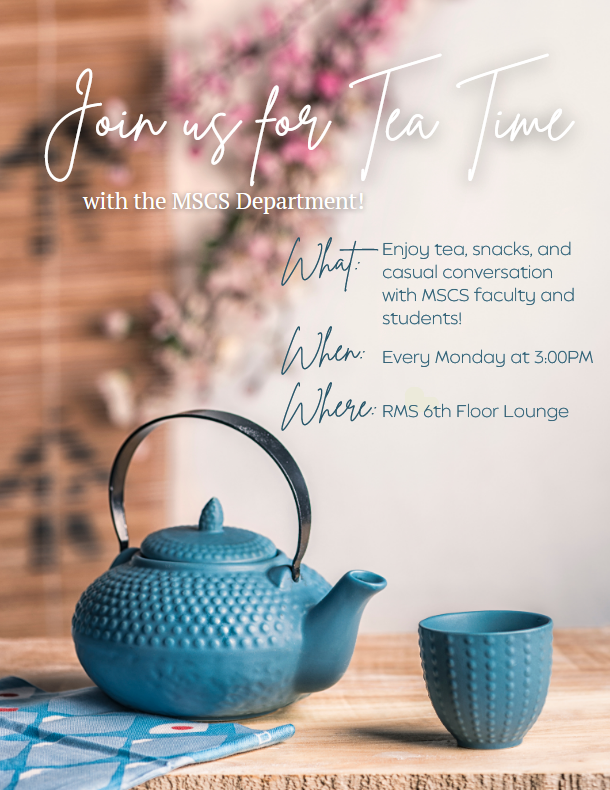
\includegraphics[scale=0.6]{images/Tea Time Poster.png}
\end{center}

\vspace{0.3in}
\noindent{\it 

\noindent{To submit an article, event, or anything else for publication in the Mess, email messeditor@stolaf.edu. Visit \href{https://wp.stolaf.edu/mscs/mscs-mess/}{http://wp.stolaf.edu/mscs/mscs-mess/} for a digital archive of previous MSCS Mess issues.}}\\
	
\hfill Name Name, Editor
	
\hfill Kyle Salois, Faculty Adviser


 

\end{document}
